%----------------------------------------------------------------------------
% Magic tutorial number W-1
%----------------------------------------------------------------------------

\NeedsTeXFormat{LaTeX2e}[1994/12/01]
\documentclass[letterpaper,twoside,12pt]{article}
\usepackage{epsfig,times}

\setlength{\textwidth}{8.5in}
\addtolength{\textwidth}{-2.0in}
\setlength{\textheight}{11.0in}
\addtolength{\textheight}{-2.0in}
\setlength{\oddsidemargin}{0in}
\setlength{\evensidemargin}{0pt}
\setlength{\topmargin}{-0.5in}
\setlength{\headheight}{0.2in}
\setlength{\headsep}{0.3in}
\setlength{\topskip}{0pt}

\def\hinch{\hspace*{0.5in}}
\def\starti{\begin{center}\begin{tabbing}\hinch\=\hinch\=\hinch\=hinch\hinch\=\kill}
\def\endi{\end{tabbing}\end{center}}
\def\ii{\>\>\>}
\def\mytitle{Magic Tutorial \#W-1: Design-Rule Extensions}
\def\q{\special{ps:(") show}\hspace*{0.6em}}
\def\bk{\special{ps:/bksp 2 string def bksp 0 92 put bksp show}\hspace*{0.4em}}

%----------------------------------------------------------------------------

\begin{document}

\makeatletter
\newcommand{\ps@magic}{%
	\renewcommand{\@oddhead}{\mytitle\hfil\today}%
	\renewcommand{\@evenhead}{\today\hfil\mytitle}%
	\renewcommand{\@evenfoot}{\hfil\textrm{--{\thepage}--}\hfil}%
	\renewcommand{\@oddfoot}{\@evenfoot}}
\newcommand{\ps@mplain}{%
	\renewcommand{\@oddhead}{}%
	\renewcommand{\@evenhead}{}%
	\renewcommand{\@evenfoot}{\hfil\textrm{--{\thepage}--}\hfil}%
	\renewcommand{\@oddfoot}{\@evenfoot}}
\makeatother
\pagestyle{magic}
\thispagestyle{mplain}


\begin{center}
  {\bfseries \Large \mytitle} \\
  \vspace*{0.5in}
  {\itshape Don Stark} \\
  \vspace*{0.5in}
   Western Research Laboratory \\
   Digital Equipment Corporation \\
   Palo Alto, CA  94301 \\
  \vspace*{0.25in}
  This tutorial corresponds to Magic version 7. \\
\end{center}
\vspace*{0.5in}

{\noindent\bfseries\large Tutorials to read first:}
\starti
   \> Magic Tutorial \#6: Design-Rule Checking \\
   \> Magic Tutorial \#9: Format Conversion for CIF and Calma \\
   \> Magic Maintainer's Manual \#2: The Technology File
\endi

{\noindent\bfseries\large Commands introduced in this tutorial:}
\starti
   \> {\itshape (None)}
\endi

{\noindent\bfseries\large Macros introduced in this tutorial:}

\starti
   \> {\itshape (None)}
\endi

\vspace*{0.25in}
\section{Introduction}

Magic's original design rule checker has proved inadequate to implement all
the rules found in advanced technologies.  The rules described
in this section allow more complicated configurations to be analyzed.
Two new rules check a region's area and its maximum width.  In addition,
width, spacing, area, and maxwidth checks may now be performed on cif layers.

\section{Area Rules}

The {\bfseries area} rule is used to check the minimum area of a region.  Its
syntax is:

\starti
   \ii {\bfseries area} {\itshape  types minarea minedge why}
\endi

{\itshape Types} is a list of types that compose the region, all of which must
be on the same plane.  
{\itshape Minarea} is the minimum area that a region must have, while {\itshape minedge}
is the minimum length of an edge for the region.  This second dimension 
is basically
an optimization to make the design rule checker run faster; without it,
the checker has to assume that a region 1 lambda wide and {\itshape minarea}
long is legal, and it must examine a much larger area when checking the
interaction between cells. Specifying {\itshape minedge} reduces this
interaction distance. An example rule is:

\starti
   \ii {\bfseries  area (emitter,em1c)/npoly 6 2 {\q}emitter must be at least 2x3{\q}}
\endi


\begin{figure}[ht]
   \begin{center}
      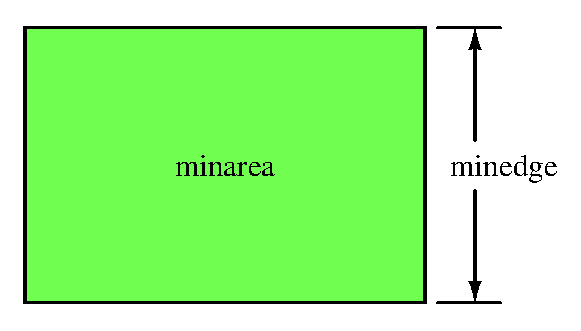
\epsfig{file=../psfigures/tutw1.2.ps, width = 0.65\columnwidth}
      \caption{Example of the area rule.}
   \end{center}
\end{figure}


\section{Maxwidth Rules}

Sometimes a technology requires that a region not be wider than a
certain value.  The {\bfseries maxwidth} rule can be used to check this.

\starti
   \ii {\bfseries maxwidth} {\itshape layers mwidth bends why}
\endi

{\itshape Layers}, the types that compose the region, must all be in the 
same plane.  The region must be less than {\itshape mwidth} wide in either the
horizontal or vertical dimension. {\itshape Bends} takes one of two values,
{\bfseries bend{\_}illegal} and {\bfseries bend{\_}ok}.  For
{\bfseries bend{\_}illegal} rules, the
checker forms a bounding box around all contiguous tiles of the correct type, 
then checks this box's width.  For example:

\starti
   \ii {\bfseries  maxwidth (emitter,em1c)/npoly 2 bend{\_}illegal\ {\bk}} \\
   \ii \>  {\bfseries {\q}emitter width cannot be over 2{\q}}
\endi

{\bfseries bend{\_}ok} rules are used to check structures where the region
must be locally less than maxwidth, but may contain bends,
T's, and X's. 

\starti
   \ii {\bfseries  maxwidth trench 2 bend{\_}ok {\q}trench must be exactly 2 wide{\q}}
\endi

{\bfseries Warning:} the bend{\_}ok rule is basically a kludge, and may fail for
regions composed of more than one type, or for intersections more
complicated than T's or X's. 
Figure~\ref{maxwidth} shows some examples of both types of rules.

\begin{figure}[ht]
   \begin{center}
      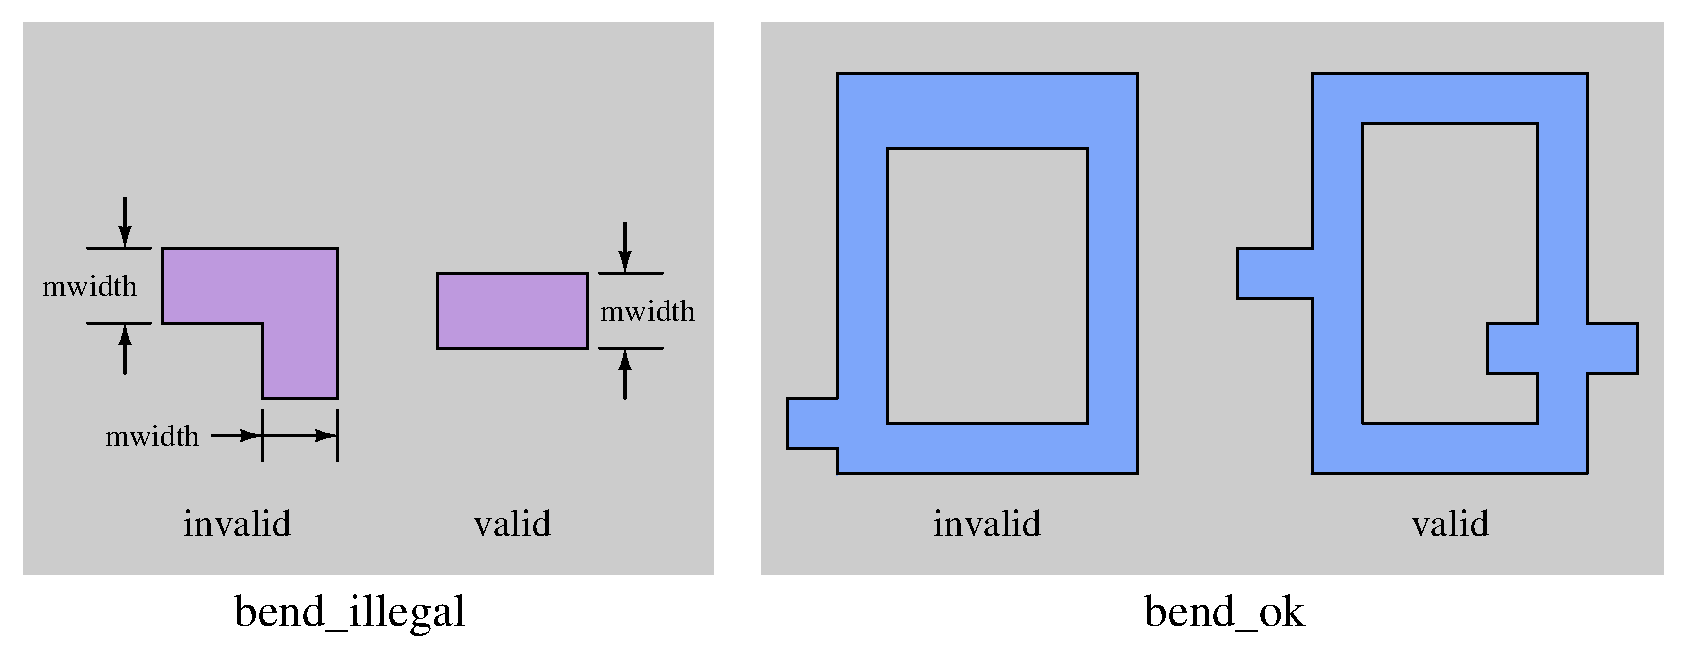
\epsfig{file=../psfigures/tutw1.1.ps, width=\columnwidth}
      \label{maxwidth}
      \caption{Examples of the maxwidth rule. The dogleg at the left would
 	be ok in a {\bfseries bend{\_}ok} rule, but fails in a
 	{\bfseries bend{\_}illegal} one, where the region's bounding
	box is checked.  For {\bfseries bend{\_}ok} rules, each tile
	in the region is checked. The left shape fails in two places:
	the top horizontal part is too thick and the stub at the bottom
	intersects the region in a shape other than a T or X.}
   \end{center}
\end{figure}

\section{Rules on CIF layers}

For technologies with complicated generated layers, it is often difficult
to check design rules on the abstract types that are drawn in Magic.  To
ameliorate this problem, the extended checker allows simple checks to be
performed on cif layers.  The rules that can be checked are width,
spacing, area, and maxarea.  Since checking rules on the cif layers
requires that these layers be generated, these checks are considerably
slower than the normal ones, and should only be used when absolutely
necessary.

\subsection{Setting the CIF style}

The {\bfseries cifstyle} rule is used to select which {\bfseries cifoutput}
style is used.

\starti
   \ii {\bfseries cifstyle} {\itshape cif{\_}style}
\endi

{\itshape Cif{\_}style} must be one of the cif styles included in the cifoutput
section.  In the current implementation, the cif checker generates all the
layers in the style regardless of whether they are actually used in
design-rule checks;  for speed, defining a separate cif style for design
rule checking it may be worthwhile when only a few layers are checked.
Any layer in the cif style, defined by either a {\itshape layer} or a
{\itshape templayer} rule, may be checked.

\subsection{Width Checks}

The syntax for {\bfseries cifwidth} is analogous to that of the regular width
rule:

\starti
   \ii {\bfseries cifwidth} {\itshape layer width why}
\endi

{\itshape Layer} is a single cif layer. (To do width checks with more than one cif
layer, {\bfseries or} all the layers into a new {\itshape templayer}). {\itshape Width}
is the minimum width of the region in centimicrons.

\subsection{Spacing Checks}

The {\bfseries cifspacing} rule is also very similar to the regular rule:

\starti
   \ii {\bfseries cifspacing} {\itshape layer1 layer2 separation adjacency why}
\endi

{\itshape Layer1} and {\itshape layer2} are both cif layers.  If
{\itshape adjacency} is {\bfseries touching{\_}ok}, then layer1 must
equal layer2. For {\bfseries touching{\_}illegal} rules, {\itshape layer1}
and {\itshape layer2} may be any two cif layers. {\itshape Separation} is
given in centimicrons.

\subsection{Area Checks}

The area rule is:

\starti
   \ii {\bfseries cifarea} {\itshape layer minarea minedge why}
\endi

{\itshape  Layer} is again a single cif layer.  {\itshape minedge} is expressed in
centimicrons, and {\itshape minarea} is given in square centimicrons.

\subsection{Maxwidth Checks}

The maxwidth rule is:

\starti
   \ii {\bfseries cifmaxwidth} {\itshape layer mwidth bends why}
\endi

Again, {\itshape layer} is a single cif layer, and {\itshape mwidth} is given in
centimicrons.

\end{document}
